\chapter{Ti-Mo-Nb-Sn-Ta-Zr Thermodynamic Database}

\section{Introduction}

The design of Ti-alloys for biomedical applications necessitates a completed thermodynamic database that will facilitate the prediction of phase compositions and fractions as a function of composition and temperature. However, there is no completed thermodynamic database for the Ti-Mo-Nb-Sn-Ta-Zr system and thus the present work aims at building a complete database with special focus on the Ti-rich alloys and bcc phase models. With this in mind the pure elements have been extensively studied and are widely adopted from the SGTE database \cite{Dinsdale1991}. The modeling of the binary systems has been widely documented with the exception of the Ta-Sn and Mo-Sn systems, while experimental phase boundary data is available for the ternary systems but little to no modeling has been completed. The Mo-Sn and Sn-Ta subsystems have high melting temperatures and little to no experimental data. In these cases, first-principles calculations based on DFT can be used to aid in modeling and supplement the lack of experimental data. The complete modeling of the Ta-Sn system is discussed in Ch3. In the present chapter, the thermodynamic descriptions of the Ti-Mo-Nb-Ta-Zr system are described. 

While many of the alloys in this Ti system have been studied experimentally, yielding phase equilibrium data, only limited calorimetry data is available. With the present work focuses on bcc Ti-rich alloys, first-principles calculations based on DFT of the enthalpy of formation of the bcc phase were calculated. The thermodynamic descriptions were built or evaluated using available experimental phase boundary data and present calculated thermochemical data. This works looks at evaluating new and previous models for the binary and Ti-containing ternary systems. 

\section{Computational details}

First-principles results based on Density Functional Theory (DFT) are used to predict the enthalpy of formation of specific phases. In the present work, the enthalpy of formation of the bcc phase was calculated for the Ti-X and Ti-X-Y (X$\neq$Y= Mo, Nb, Ta, Zr) using the calculated energy of the pure elements in their SER states. For each Ti-containing binary system at least 5 composition energy structures were calculated and three compositions for the Ti-containing ternary system. For each system, three special quasirandom structures (SQS) of varying compositions were relaxed to get an accurate representation of the enthalpy of formation across the composition range. For the binary phases the compositions are each 16-atom unit cells at Ti$_4$X$_{12}$, Ti$_8$X$_8$, and Ti$_{12}$X$_4$ and the ternary phase compositions of Ti$_{12}$X$_{12}$Y$_{12}$ (36-atom), Ti$_{16}$X$_8$Y$_8$ (32-atom), Ti$_{48}$X$_8$Y$_8$ (64-atom) structures are used with one X$_8$Y$_8$ (16-atom), where X and Y are the alloying elements. These SQS in the bcc phase that were implemented were developed by Jiang et al. \cite{Jiang2004,Jiang2009}. Relaxation of these structures is complicated and explained in the methodology section. The DFT calculations are completed using VASP (Vienna ab-initio Simulation Package) \cite{Kresse1996}. The ion-electron interactions were described using the projector augmented wave (PAW) \cite{Kresse1999,Blochl1994} method with the exchange-correlation (X-C) functional implemented by Perdew, Burke, and Ernzerhof (PBE) \cite{Perdew1996a}. For consistency, a 310 eV energy cutoff was adopted for all calculations, which is roughly 1.3 times higher than the default value. The energy convergence criterion was 10-6 eV/atom, and the Monkhorst-Pack scheme is used for Brillouin zone sampling \cite{Kresse1996,Monkhorst1976a}. 

\section{Binary systems}

In order to build the database, as discussed above, the pure elements were adapted from the SGTE database \cite{Dinsdale1991}. After the incorporation of the pure elements, all the binary systems were then evaluated. When applicable, previous models of the binary systems were evaluated for accuracy and model compatibility and incorporated into the database. After incorporation of all binary systems, the Ti-containing ternary systems were evaluated, with the exception of Mo-Nb-Ta which had a previous model available by Xiong et al. \cite{Xiong2004} and was incorporated into this work. To do the binary and ternary evaluations, the enthalpy of formation of the bcc phase for the Ti-containing alloys was calculated across the composition ranges. To calculate the enthalpy of formation of the bcc phase, the enthalpy of the pure elements had to be calculated in their standard element reference states (SER). The phases and results are listed in Table \ref{Ch3-table:pspureele}. In order to ensure the accuracy of the calculations, the bulk modulus \textit{B} calculated in the present work was compared with the experimental data. The experimental \textit{B} varied on average by 1 GPa from the calculated \textit{B}. This discrepancy is not large and is attributed with the temperature difference thus these calculations prove to be accurate. 

The previous thermodynamic descriptions for the Ti-containing binaries were evaluated with experimental data as well as looking at the enthalpy of formation of the bcc phase using present first-principles calculations. The enthalpy of formation of the bcc phase calculated for each Ti-containing binary from first-principles is listed in Table \ref{Ch3-table:hof}. 



\subsection{Ti-Mo}

The Ti-Mo binary evaluation was taken from the COST 507 database and the thermodynamic description was evaluated by Saunders \cite{Ansara1998}. This model was chosen because it is the modeled incorporated into the Ti-Mo-Zr modeling done by Kar et al. \cite{Kar2008}. Interaction parameters were evaluated for the liquid, fcc (face centered cubic), hcp, bcc$\#$1, bcc$\#$2 ordered and disordered phases, AlM-D019, AlM-D022, and the AlTi-L10 phases. Figure \ref{Ch3-figure:TiMo}a shows the comparison of the available phase boundary data from Murray et al. \cite{Murray1981} with the Saunders model. The phase boundary data is reproduced in the with the Saunders model. Figure \ref{Ch3-figure:TiMo}b shows the enthalpy of formation of the bcc phase predicted from the model at 300 K compared with the present first-principles results at 0 $^\circ$K. The enthalpy of formation of the bcc phase predicted varies from the first-principles calculations drastically between 20 and 80 at $\%$ Mo. This discrepancy is seen due to the disagreement on the existence of a bcc miscibility gap. Previous research has shown the need for a bcc miscibility gap which would fit what is seen in the first-principles calculations \cite{Predel1997,Hoffman1967}. Kar et al. showed that the experimental data from higher-component systems fit better with the description containing no miscibility gap. Based on this, the model by Saunders was adopted for the database with no changes. 

\subsection{Ti-Nb}

The Ti-Nb binary evaluation was taken from Zhang et al. \cite{Zhang2001} and plotted in Figure \ref{Ch3-figure:TiNb}a. Originally the binary evaluation was taken from Kumar et al. \cite{Kumar1994}. The figure shows solidus data ($\square$) and hcp and bcc solvus data ($\circ$) used in the Kumar et al. evaluation. The model from Kumar was used in the modeling of the Ti-Nb-Zr. The phase diagram was evaluated using phase boundary data on the Ti-rich side and liquidus data. Not only was the binary evaluation adapted due to the use in the Ti-Nb-Zr ternary but it also reproduced the experimental phase boundary data reasonably well. However, the model was changed to the new model by Zhang et al. ($\triangle$) due to the new phase boundary data on the Nb rich side. The present first-principles calculations of the enthalpy of formation of the bcc phase are plotted in Figure \ref{Ch3-figure:TiNb}b. The present DFT results (circles) are at 0 $^\circ$K while the CALPHAD prediction (solid line) is at 300 $^\circ$K which explains the average variance of 0.17 kJ/mol-atom between the DFT and CALPHAD predictions. However, even with the variance the CALPHAD prediction compares well with the DFT results and the sublattice models are similar to the database being built. With the reproduction of experimental data and the first-principles results no alterations were made to the thermodynamic evaluation.

\subsection{Ti-Ta}

The Ti-Ta binary was taken from the COST 507 database and evaluated by Saunders \cite{Ansara1998}. The phase diagram is shown in Figure \ref{Ch3-figure:TiTa}a. The figure is plotted with liquidus and solidus experimental data ($\lozenge$, Y) as well as bcc and hcp solvus data ($\triangle$, $\square$, $\circ$). The evaluation includes interaction parameters for the fcc, hcp, liquid, AlM-D019, AlM-D022, AlTi-L10 and the bcc$\#$1 and bcc$\#$2 ordered and disordered phases. The thermodynamic description reproduces the phase boundary experimental data from Murray et al. \cite{Murray1987}. The first-principles results (circles) and the enthalpy of formation of the bcc phase predicted by the CALPHAD modeling is shown in Figure \ref{Ch3-figure:TiTa}b. The CALPHAD prediction of the enthalpy of formation reproduces the results from first-principles reasonably well on the Ti-rich and Ta-rich sides. The first-principles results between 10 and 60 at $\%$ Ta vary on an average by 0.17 kJ/mol-atom. However, the CALPHAD prediction is at 300 $^\circ$K and the first-principles are at 0 $^\circ$K which explains the variance and the CALPHAD prediction follows the same trend that is seen in the first-principle results. The modeling and sublattices used were compatible with the database being built and thus the thermodynamic description by Saunders was not altered. 

\subsection{Ti-Zr}

The thermodynamic description of the Ti-Zr alloy system evaluated by Kumar et al. \cite{Kumar1994a} is used in the present work. The model by Kumar et al. was used in the ternary modeling of the Ti-Mo-Zr and Ti-Nb-Zr ternary alloys. The sublattice modeling was consistent with the previous binary systems. The evaluation introduced interaction parameters for the liquid, bcc, and hcp solution phases. Figure \ref{Ch3-figure:TiZr}a plots the evaluation compared with phase boundary data for the bcc to hcp phase ($\circ$) transformation and solidus ($\lozenge$). The thermodynamic description accurately reproduces the phase boundary data. The evaluation also included heat of transformation data shown in the paper by Kumar et al. \cite{Kumar1994a}. Figure \ref{Ch3-figure:TiZr}b plots the first-principles results (circles) versus the CALPHAD prediction (solid line) for the enthalpy of formation of the bcc phase. The DFT results and CALPHAD modeling vary on average by 1.2 kJ/mol-atom. The variance is larger than the other binary alloys due to the instability of the bcc phase at both 0 $^\circ$K and 300 $^\circ$K for the Ti-Zr alloy but the calculations and CALPHAD prediction follow the same trend. Based on the agreement between the experimental data, first-principles and CALPHAD prediction no alterations were made to the thermodynamic description. 

\subsection{Non Ti-containing binaries}

Figure \ref{Ch3-figure:binary1} shows the evaluation of the Mo-Nb, Mo-Ta, and Nb-Ta alloys. The Mo-Nb, Mo-Ta and Nb-Ta binary descriptions were adapted from the Mo-Nb-Ta ternary paper by Xiong et al. \cite{Xiong2004}. Xiong et al. introduced binary interaction parameters for the liquid and bcc solution phases. The Mo-Nb evaluation was completed using differential thermal analysis experiments that measured both the liquidus and solidus temperature. Multiple authors measured experiments and Xiong et al. picked the experiments (shown in the figure as X, +) that estimated the pure elements reasonably well to build the evaluation on. Xiong et al. saw that the experiments shown by $\circ$, $\triangle$, $\square$ agreed well with the thermodynamic description. The remaining work ($\lozenge$, *) was too low and thus wasn’t included in the evaluation of the binary alloy. The Mo-Ta alloy evaluation was done using two sets of experimental data ($\triangle$,* , $\lozenge$, $\square$) for the evaluation that agree well with the accepted melting temperatures of Mo and Ta. The remaining experimental data ($\circ$) was higher than the other experimental work by 70 $^\circ$C and thus was not used for the evaluation. The Nb-Ta binary evaluation was done using the melting temperature experimental data ($\circ$, $\triangle$, $\square$) because it predicted the melting temperatures of Nb and Ta accurately. The remaining experimental work which measured the solidus temperature (*) was not used because the melting temperatures of Nb and Ta showed discrepancy. The remaining experimental work ($\lozenge$) was not included in the evaluation because similarly to the Mo-Ta alloy the experimental work was 70 $^\circ$C higher than the other work. These three evaluations were chosen because these binaries were evaluated to make up the Mo-Nb-Ta ternary alloy and the modeling was done consistently using the same sublattices models. The evaluations fit well with available experimental data and thus they can be added to the database without any changes.

Figure \ref{Ch3-figure:binary2} shows the Mo-Zr, Nb-Zr, and Ta-Zr alloys. For the Mo-Zr binary alloy system, there were multiple previous thermodynamic descriptions and experimental results available. In the present work, the evaluation by Perez et al. \cite{Perez2003} was chosen. The experimental data plotted was determined for the single-phase region, two-phase region, phase boundaries and peritectic and eutectiod reactions. Perez et al. goes into more detail on the available experimental data and was included in the evaluation of the thermodynamic description. The thermodynamic description generally reproduces all experimental data and is compatible with the sublattice modeling used in the database. The Perez et al. model was also incorporated into the Ti-Mo-Zr ternary modeling. Perez et al. introduced interaction parameters for the liquid, bcc, hcp and MZr$_2$ (laves$\_$c15) phases. The Nb-Zr alloy thermodynamic description evaluated by Guillermet \cite{Guillermet1991} was chosen for the present work. The figure shows the solidus experimental data ($\lozenge$, *) as well as the hcp solvus (Y, $\circ$)and bcc miscibility gap ($\square$, +, $\triangle$)data. The description includes interaction parameters for the liquid, bcc and hcp solution phases. The thermodynamic description was chosen because it was the description that Kumar et al. \cite{Kumar1994a} included in his modeling of the Ti-Nb-Zr alloy system. The experimental phase boundary and liquidus data from Abriata et al. \cite{Abriata1982} fits well with the model. The Ta-Zr binary evaluated by Guillermet \cite{Guillermet1995} was chosen for the present database. As Guillermet discusses there was quite a lot of experimental data, shown in the figure. Guillermet discusses the experimental data more in his paper. The figure plots single-phase, two-phase, phase boundary, and solidus experimental data. Interaction parameters were introduced for the bcc, hcp and liquid phases. Guillermet had phase boundary results from at least 5 different authors and thermodynamic results from three different authors. The evaluation reproduced the data fairly well. The sublattice modeling fit with the database and thus this binary was selected.The interaction parameters for all the binary systems are listed in Table \ref{table:ip}.

\section{Ti-containing ternary sections}

\subsection{Ti-Mo-Nb}

A thermodynamic description for the Ti-Mo-Nb ternary system has never been evaluated. Two experimental investigations were done on the Ti-Mo-Nb system at 873 $^\circ$K and 1373 $^\circ$K \cite{English1961,Prokoshkin1967}. While both investigations agree that the isothermal section at 1373 $^\circ$K is solely the bcc phase, the investigations differed on the phase boundary data at 873 $^\circ$K. It is suspected that at such a low temperature the samples did not reach equilibrium which accounts for the discrepancy. Based on this, the binary interpolation of the isothermal sections at 1373 $^\circ$K and 873 $^\circ$K were plotted. The phase diagram at 1373 $^\circ$K agreed with the experimentally determined phase diagram to be solely the bcc phase. The phase diagram at 873 $^\circ$K is plotted in Figure \ref{Ch3-figure:TiMoNb}a. The discrepancy at 873 $^\circ$K, is the existence of the bcc miscibility gaps as well as what compositions the phase boundary lines lie at. First-principles calculations of the enthalpy of formation of the bcc phase are plotted against the binary interpolation in Figure \ref{Ch3-figure:TiMoNb}b. While the first-principles calculations are at 0 $^\circ$K and the binary interpolation is at 300 $^\circ$K the calculation results are reproduced with the CALPHAD prediction. The prediction varies by less than 1.5 kJ/mol-atom for all the calculations except at Mo$_{0.5}$Nb$_{0.5}$. While the calculation varies substantially from the prediction at Mo$_{0.5}$Nb$_{0.5}$, in order to improve this, the Mo-Nb binary system would have to be adjusted. In the present work, no thermochemical data was used to ensure the accuracy of the non Ti-containing binary systems but the previous binary models were able to reproduce the phase boundary data as discussed above. Based on the discrepancy between the experimental data and the fact that the thermochemical first-principles calculations are reproduced well by the binary interpolation, no ternary interaction parameters were evaluated. 

\subsection{Ti-Mo-Ta}

The thermodynamic description of the Ti-Mo-Ta alloys system had not been previously modeled. The binary interpolation of the Ti-Mo-Ta alloy is plotted in Figure \ref{Ch3-figure:TiMoTa1}a at 873 $^\circ$K and compared with experimental data from Nikitin et al. \cite{Nikitin1971}. At 873 $^\circ$K, the Ti-Mo-Ta alloy has the bcc and hcp solution phases. The experimental data showed a two-phase bcc-hcp region in the Ti-rich corner, while the binary interpolation shows a bcc miscibility gap which forms a tie triangle with the hcp phase. Figure \ref{Ch3-figure:TiMoTa1}b shows the first-principles calculations (circles) of the enthalpy of formation of the bcc phase compared with the binary interpolation from the CALPHAD prediction. The first-principles calculations line up fairly well with the CALPHAD prediction. However, due to the discrepancy of the experimental data, ternary interaction parameters were evaluated using the experimental and first-principles results. Interaction parameters for the hcp and bcc phases were investigated. The evaluated interaction parameters are listed in Table \ref{Ch3-table:ip}. After assessing the ternary interaction parameters, the isothermal section was again plotted and compared with experimental data in Figure \ref{Ch3-figure:TiMoTa2}a and the enthalpy of formation of the newly assessed bcc phase is plotted as a dashed line in Figure \ref{Ch3-figure:TiMoTa1}b. The assessment reproduces the first-principles results. With the introduction of the interaction parameters the isothermal section fits with the experimental data. Figure \ref{Ch3-figure:TiMoTa2}b is zoomed in on the Ti-rich corner. The work by Nikitin determined hcp phase boundary data plotted as ($\circ$) and two phase experimental data as $\LEFTcircle$. The two phase experimental data is reproduced by the current model. The hcp phase boundary data is not reproduced. However, reliable solid phase boundary data is difficult to obtain at such a low temperature and if the evaluation is altered to fit the data it then over fits and stabilizes non-equilibrium phases. 

\subsection{Ti-Mo-Zr}

The thermodynamic description of the Ti-Mo-Zr alloy system was previously modeled by Kar et al. \cite{Kar2008}. The same binary phases used in the modeling by Kar et al. were included in the database. The phases in this system are liquid, bcc, hcp and laves$\_$c15. After interpolating the ternary system from the binary models and comparing to two sets of available experimental data, Kar et al. introduced interaction parameters for the laves$\_$c15 phase. Using the model by Kar et al., the present work plotted the ternary isothermal section at 1273 $^\circ$K comparing to phase boundary data plotted in Figure \ref{Ch3-figure:TiMoZr}a. As discussed by Kar et al. there is phase boundary data from two authors. The sets of phase boundary data conflict on how far out the two-phase region should extend toward the Ti-rich corner and whether there is a bcc miscibility gap. After plotting the data, Kar et al. decided not to introduce any bcc, liquid or hcp interaction parameters. Only one set of phase boundary data is plotted \cite{Prokoshkin1967}. The phase boundary data fits well on the Zr-Mo binary side. The predicted enthalpy of formation of the bcc phase is plotted with the first-principles results in Figure \ref{Ch3-figure:TiMoZr}b. The first-principles results vary on average by 0.025 kJ/mol-atom. Based on the available experimental data, first-principles calculations and the conclusions from Kar et al. the present work agrees with the introduction of the ternary laves$\_$c15 interaction parameters and lack of liquid, bcc and hcp ternary interaction parameters. The ternary laves$\_$c15 interaction parameters are listed in Table \ref{Ch3-table:ip}.

\subsection{Ti-Nb-Ta}

A thermodynamic description of the Ti-Nb-Ta had not been evaluated but different isothermal sections had been estimated by Na et al. \cite{Na2001} using phase boundary data. The phase boundary data was obtained through XRD. Na et al. looked at samples at 823 $^\circ$K and 673 $^\circ$K. The authors discussed that it is likely that the alloys at 673 $^\circ$K never reached equilibrium conditions. The experimental results were plotted on the binary interpolation in Figure \ref{Ch3-figure:TiNbTa1}a and Figure \ref{Ch3-figure:TiNbTa1}b. The bcc phase boundary data does not match with the binary interpolation. Figure \ref{Ch3-figure:TiNbTa1}c plots the enthalpy of formation of the bcc phase predicted by the CALPHAD modeling and compared with the first-principles results. The first-principles results vary from the CALPHAD prediction. The variance of the first-principles results and the variance of the experimental data lead to the evaluation of ternary interaction parameters for the bcc and hcp phases. The evaluation was done using the 823 $^\circ$K experimental data and first-principles calculations. Due to the conclusion by Na et al. that the 673 $^\circ$K samples did not reach equilibrium the data was neglected during the evaluation. The evaluation led to only one bcc ternary interaction parameter needed and it is listed in Table \ref{Ch3-table:ip}. After evaluation, the ternary isothermal sections are plotted with the phase boundary data in Figure \ref{Ch3-figure:TiNbTa2}a and Figure \ref{Ch3-figure:TiNbTa2}b. The isothermal sections at both 673 and 823 $^\circ$K reproduces the experimental data reasonably well. The prediction of the enthalpy of formation of the bcc phase also improved to accurately predict the first-principles results.

\subsection{Ti-Nb-Zr}

The Ti-Nb-Zr was previously evaluated by multiple authors. In the present work the ternary isothermal sections were compared with work by Kumar et al. \cite{Kumar1994a} and Tokunaga et al. \cite{Tokunaga2007}. The Ti-Zr and Nb-Zr binary alloys were the same modeled binaries as chosen by Kumar et al. The Ti-Nb binary however was changed to a newer evaluation by Zhang et al. \cite{Zhang2001} which was discussed above. In the evaluation done by Kumar et al. \cite{Kumar1994a}, the liquidus projection and various isothermal sections were interpolated from the binary alloys but not compared with experimental data. In the present work, the binary interpolation was used to plot the isothermal sections at the same temperature as Kumar et al. The ternary isothermal sections varied due to the change in the Ti-Nb binary. The binary interpolation of the isothermal section at 843 $^\circ$K is plotted in Figure \ref{Ch3-figure:TiNbZr}a and compared with experimental data for the tie triangle ($\triangle$) and two-phase region (\Leftcircle) shown in the paper by Tokunaga et al. \cite{Tokunaga2007}. The binary interpolation reproduced the hcp and bcc disordered and ordered tie triangle phase boundary data and the two-phase bcc miscibility gap region. The enthalpy of formation of the bcc phase is plotted in Figure \ref{Ch3-figure:TiTa}b. The CALPHAD prediction varies on an average by 1.34 kJ/mol-atom. While it the CALPHAD prediction varies more drastically than the other enthalpies of formation from the calculated first-principles results, it follows the same trend and fits well with the experimental data. So, the conclusion was reached to not introduce ternary interaction parameters.  

\subsection{Ti-Ta-Zr}

For the Ti-Ta-Zr alloys system, Lin et al. \cite{Lin1996} calculated the isothermal sections using binary interpolations and introduced no interaction parameters. The isothermal sections at 1273 and 1773 $^\circ$K are plotted in Figure \ref{Ch3-figure:TiTaZr}a and Figure \ref{Ch3-figure:TiTaZr}b. Experimental phase boundary data ($\circ$) along the bcc miscibility gap at 1273 $^\circ$K and single phase $\CIRCLE$ and two phase region $\LEFTcircle$ data using x-ray diffraction at 1773 $^\circ$K are plotted to compare with the binary interpolation \cite{Lin1996,Hoch1964}. The phase boundary data is reproduced excellently. The single-phase data fits well with the interpolation with the two-phase region falling on the phase boundary line. Figure \ref{Ch3-figure:TiTaZr}c is the enthalpy of formation of the bcc predicted from first-principles calculations and the binary interpolation. On average the first-principles varies by 3.69 kJ/mol-atom. While this variance is larger than other plots it can be attributed to the temperature difference and instability of the bcc phase at 300 $^\circ$K and 0 $^\circ$K. Since the experimental data is reproduced, it was concluded that no overfitting to the first-principles calculations was needed and thus none were evaluated. 
After evaluation, the thermodynamic descriptions of all the binary systems and Ti-containing ternary systems are listed in Table \ref{Ch3-table:ip} and combined into a single tdb database in the appendix.

\section{Conclusion}

The present work builds a thermodynamic database for the Ti-Mo-Nb-Ta-Zr system using descriptions of the pure elements, binary systems and Ti-containing ternary systems. The thermodynamic descriptions of the pure elements was adapted from the SGTE database \cite{Dinsdale1991}. The previous models for the binary systems were evaluated for compatibility and accuracy. With the present application focusing on Ti-alloys, first-principles results for the enthalpy of formation of the bcc phase was used to ensure the accuracy of the thermodynamic descriptions in predicting thermochemical data. Binary interpolations were predicted for the Ti-containing ternary systems and compared with isothermal experimental data as well as first-principles of enthalpy of formation of the bcc phase. When needed the ternary interaction, parameters were evaluated. The compatible thermodynamic descriptions were complied into a single tdb database. The raw first-principles data as well as the tdb database are in appendix A. 


\newpage
\begin{table}[H]
	\caption{Bulk modulus \textit{B} and enthalpy are listed for each pure element in their SER phase listed. The sv and pv refer to the electrons chosen as valance according to the VASP recommendations. The results are compared with available experimental data.}
	\centering
	\begin{tabular}{ c c c c c }
		\hline
		Pure Elements & Reference & Phase & Enthalpy (kJ/mol-atom) & \textit{B} (GPa) \\
		\hline
		Ti$\_$sv & Shang \cite{Shang2010b} & hcp & -7.89 & 113\\
                 & Expt 300 K \cite{WolframResearch} & & & 110\\
        Mo$\_$pv & This work 0 K & bcc & -10.84 & 262\\
                        & Expt 300 K \cite{Dickinson1967a} & & & 261\\
        Nb$\_$sv & This work & bcc & -10.22 & 171\\
                       & Expt 300 K \cite{Bolef1961} & & & 172\\
         Ta$\_$pv & This work 0 K & bcc & -11.85 & 196\\
                       & Expt 300 K \cite{Bolef1961} & & & 196\\
          Zr$\_$sv & Shang 0 K \cite{Shang2010b} & hcp & -8.51 & 94\\
                        & Calc 0 K \cite{Treco1953_964,Bergerhoff1983,Karlsruhe,MaterialsProject} & & & 94\\
		\hline
	\end{tabular}
	\label{Ch3-table:pspureele}
\end{table}
\clearpage
%%%

\newpage
\begin{longtable}[H]{ c c c c }
	\caption{First-principles calculations of the enthalpy of formation of the bcc phase in kJ/mol-atom for different atomic percent compositions of the Ti-X binary systems at 0 K.} 	\label{Ch3-table:hof} \\
		\hline
		BCC Phase 0 K & x(Ti) & x(X) & HForm (kJ/mol-atom)\\
		\hline
        \endhead
        \hline
        \endfoot
		Ti & 1.000 & 0.000 & 7.29\\
		Ti15Mo & 0.937 & 0.063 & 3.08\\
		Ti7Mo & 0.875 & 0.125 & 2.82\\
		Ti75Mo25 & 0.750 & 0.250 & 1.12\\
		Ti50Mo50 & 0.500 & 0.500 & -3.67\\
		Ti25Mo75 & 0.250 & 0.750 & -5.18\\
		TiMo15 & 0.063 & 0.937 & 1.79\\
		TiMo53 & 0.019 & 0.981 & 5.82\\
		Mo & 0.000 & 1.000 & 0.00\\
		Ti53Nb & 0.981 & 0.019 & 6.92\\
		Ti7Nb & 0.875 & 0.125 & 5.88\\ 
		Ti75Nb25 & 0.750 & 0.250 & 7.57\\
		Ti50Nb50 & 0.500 & 0.500 & 8.54\\
		Ti25Nb75 & 0.250 & 0.750 & 1.15\\
		TiNb15 & 0.063 & 0.938 & 0.59\\
		TiNb53 & 0.019 & 0.981 & 0.20\\
		Nb & 0.000 & 1.000 & 0.00\\
		Ti53Ta & 0.981 & 0.019 & 7.21\\
		Ti15Ta & 0.938 & 0.063 & 7.04\\
		Ti7Ta & 0.875 & 0.125 & 9.28\\
		Ti75Ta25 & 0.750 & 0.250 & 4.89\\
		Ti50Ta50 & 0.500 & 0.500 & 3.94\\
		Ti25Ta75 & 0.250 & 0.750 & 3.10\\
		TiTa15 & 0.063 & 0.938 & 0.94\\
		TiTa53 & 0.019 & 0.981 & 0.28\\
		Ta & 0.000 & 1.000 & 0.00\\
		Ti53Zr & 0.981 & 0.019 & 5.49\\
		Ti75Zr25 & 0.750 & 0.250 & 4.59\\
		Ti50Zr50 & 0.500 & 0.500 & 1.94\\
		Ti25Zr75 & 0.250 & 0.750 & 3.50\\
		TiZr15 & 0.063 & 0.938 & 5.72\\
		Zr & 0.000 & 1.000 & 8.19\\
		\hline
\end{longtable}
%%%

\newpage
\begin{longtable}[H]{ c c c }
	\caption{Thermodynamic parameters for the Ti-Mo-Nb-Ta-Zr system. The thermodynamic description of the pure elements is not included. The pure elements were adopted from the SGTE database and are listed in the supplementary tdb file \cite{Long1998a}.}	\label{Ch3-table:ip}\\
		\hline
		Phase & Reference & Interaction Parameter\\
		\hline
		\endhead
		\hline
		\endfoot
		Liquid & \cite{Ansara1998} & $0^\textit{L}_{Ti,Mo} = -9000.0+2.00*T$\\
		          & \cite{Zhang2001} & $0^\textit{L}_{Ti,Nb} = 7406.1$\\
		          & \cite{Ansara1998} & $0^\textit{L}_{Ti,Ta} = 1000.0$\\
		          & \cite{Ansara1998} & $0^\textit{L}_{Ti,Ta} = -7000.0$\\
		          & \cite{Kumar1994a} & $0^\textit{L}_{Ti,Zr} = -967.7$\\
		          & \cite{Xiong2004} & $0^\textit{L}_{Mo,Nb} = 15253.7$\\
		          & \cite{Xiong2004} & $1^\textit{L}_{Mo,Nb} = 10594.2$\\
		          & \cite{Xiong2004} & $0^\textit{L}_{Mo,Ta} = 13978.9$\\
		          & \cite{Perez2003} & $0^\textit{L}_{Mo,Zr} = -24055.1+8.146*T$\\
		          & \cite{Perez2003} & $1^\textit{L}_{Mo,Zr} = -5132.17+4.804*T$\\
		          & \cite{Guillermet1991} & $0^\textit{L}_{Nb,Zr} = 10311.0$\\
		          & \cite{Guillermet1991} & $1^\textit{L}_{Nb,Zr} = 6709.0$\\
		          & \cite{Guillermet1995} & $0^\textit{L}_{Ta,Zr} = 13832.1$\\
		          & \cite{Guillermet1995} & $1^\textit{L}_{Ta,Zr} = -7150$\\
          BCC & \cite{Ansara1998} & $0^\textit{L}_{Ti,Mo} = 2000.0$\\
                  & \cite{Ansara1998} & $1^\textit{L}_{Ti,Mo} = -2000.0$\\
                  & \cite{Zhang2001} & $0^\textit{L}_{Ti,Nb} = 13045.3$\\
                  & \cite{Ansara1998} & $0^\textit{L}_{Ti,Ta} = 12000.0$\\
                  & \cite{Ansara1998} & $1^\textit{L}_{Ti,Ta} = -2500.0$\\
                  & \cite{Kumar1994a} & $0^\textit{L}_{Ti,Zr} = -4346.2+5.49*T$\\
                  & \cite{Xiong2004} & $0^\textit{L}_{Mo,Nb} = -68202.6+29.86*T$\\
                  & \cite{Xiong2004} & $1^\textit{L}_{Mo,Nb} = 8201.3$\\
                  & \cite{Xiong2004} & $0^\textit{L}_{Mo,Ta} = -75129.2+30.00*T$\\
                  & \cite{Xiong2004} & $1^\textit{L}_{Mo,Ta} = 6039.2$\\
                  & \cite{Perez2003} & $0^\textit{L}_{Mo,Zr} = 17936.0+3.10*T$\\
                  & \cite{Perez2003} & $1^\textit{L}_{Mo,Zr} = -991.0+4.30*T$\\
                  & \cite{Xiong2004} & $0^\textit{L}_{Nb,Ta} = 1298.0$\\
                  & \cite{Guillermet1991} & $0^\textit{L}_{Nb,Zr} = 15911.0+3.35*T$\\
                  & \cite{Guillermet1991} & $1^\textit{L}_{Nb,Zr} = 3919.0-1.09*T$\\
                  & \cite{Guillermet1995} & $0^\textit{L}_{Ta,Zr} = 29499.6+2.67*T$\\
                  & \cite{Guillermet1995} & $1^\textit{L}_{Ta,Zr} = -4396.2+4.43*T$\\
                  & \cite{Guillermet1995} & $2^\textit{L}_{Ta,Zr} = -6353.3+4.91*T$\\
                  & This work & $0^\textit{L}_{Ti,Mo,Ta} = -154731.2$\\
                  & This work & $0^\textit{L}_{Nb,Ta,Ti} = -136603.3$\\
                  & This work & $1^\textit{L}_{Nb,Ta,Ti} = -136602.7$\\
          HCP & \cite{Ansara1998} & $0^\textit{L}_{Ti,Mo} = 22760.0-6.00*T$\\      
                  & \cite{Zhang2001} & $0^\textit{L}_{Ti,Nb} = 11742.4$\\
                  & \cite{Ansara1998} & $0^\textit{L}_{Ti,Ta} = 8500.0$\\
                  & \cite{Kumar1994a} & $0^\textit{L}_{Ti,Zr} = 5133.0$\\
                  & \cite{Perez2003} & $0^\textit{L}_{Mo,Zr} = 26753.8+4.56*T$\\
                  & \cite{Guillermet1991} & $0^\textit{L}_{Nb,Zr} = 24411.0$\\
                  & \cite{Guillermet1995} & $0^\textit{L}_{Ta,Zr} = 30051.7$\\
           FCC & \cite{Ansara1998} & $0^\textit{L}_{Ti,Mo} = 16500.0$\\
                  & \cite{Ansara1998} & $0^\textit{L}_{Ti,Ta} = 8500.0$\\
    Al3M$\_$D022 & \cite{Ansara1998} & $0^\textit{L}_{Ti:Ti} = 4*GFCCTI$\\
                            & \cite{Ansara1998} & $0^\textit{L}_{Mo:Mo} = 4*GFCCMO$\\
                            & \cite{Ansara1998} & $0^\textit{L}_{Ti:Mo} = GFCCMO+3.0*GFCCTI$\\
                            & \cite{Ansara1998} & $0^\textit{L}_{Mo:Ti} = 3.0*GFCCMO+GFCCTI$\\
                            & \cite{Ansara1998} & $0^\textit{L}_{Ti:Ta} = GFCCTA+3.0*GFCCTI$\\
         AlM$\_$D019 & \cite{Ansara1998} & $0^\textit{L}_{Ti:Ti} = 4.0+4.0*GHSERTI$\\
                              & \cite{Ansara1998} & $0^\textit{L}_{Mo:Mo} = 4.0*GHCPMO$\\
                              & \cite{Ansara1998} & $0^\textit{L}_{Ta:Ta} = 4.0*GHCPTA$\\
                              & \cite{Ansara1998} & $0^\textit{L}_{Ti:Mo} = 17072.0-4.5*T+GHCPMO+3.0*GHSERTI$\\
                              & \cite{Ansara1998} & $0^\textit{L}_{Mo:Ti} = 17072.0-4.5*T+3.0*GHCPMO+GHSERTI$\\
                              & \cite{Ansara1998} & $0^\textit{L}_{Ti:Ta} = 6376.0+GHCPTA+3.0*GHSERTI$\\
                              & \cite{Ansara1998} & $0^\textit{L}_{Ta:Ti} = 6376.0+3.0*GHCPTA+GHSERTI$\\
                              & \cite{Ansara1998} & $0^\textit{L}_{Ti:Mo} = 51212.0-13.5*T$\\
                              & \cite{Ansara1998} & $0^\textit{L}_{Mo,Ti:Ti} = 51212.0-13.5*T$\\
                              & \cite{Ansara1998} & $0^\textit{L}_{Mo:Mo,Ti} = 5692.0-1.5*T$\\
                              & \cite{Ansara1998} & $0^\textit{L}_{Ti:Ti,Mo} = 5692.0-1.5*T$\\
                              & \cite{Ansara1998} & $0^\textit{L}_{Ta,Ti:Ta} = 19128.0$\\
                              & \cite{Ansara1998} & $0^\textit{L}_{Ta,Ti:Ti} = 19128.0$\\
                              & \cite{Ansara1998} & $0^\textit{L}_{Ta:Ta,Ti} = 2128.0$\\
                              & \cite{Ansara1998} & $0^\textit{L}_{TI:Ta,Ti} = 2128.0$\\
                       AlTi & \cite{Ansara1998} & $0^\textit{L}_{Ti:Ti} = 2.0*GFCCTI$\\
                              & \cite{Ansara1998} & $0^\textit{L}_{Mo:Mo} = 2.0*GFCCMO$\\
                              & \cite{Ansara1998} & $0^\textit{L}_{Ta:Ta} = 2.0*GFCCTA$\\
                              & \cite{Ansara1998} & $0^\textit{L}_{Ti:Mo} = 8250.0+GFCCMO+GFCCTI$\\
                              & \cite{Ansara1998} & $0^\textit{L}_{Mo:Ti} = 8250.0+GFCCMO+GFCCTI$\\
                              & \cite{Ansara1998} & $0^\textit{L}_{Ti:Ta} = 4250.0+GFCCTA+GFCCTI$\\
                              & \cite{Ansara1998} & $0^\textit{L}_{Ta:Ti} = 4250.0+GFCCTA+GFCCTI$\\
                              & \cite{Ansara1998} & $0^\textit{L}_{Mo,Ti:Mo} = 8250.0$\\
                              & \cite{Ansara1998} & $0^\textit{L}_{Mo,Ti:Ti} = 8250.0$\\
                        & \cite{Ansara1998} & $0^\textit{L}_{Mo:Mo,Ti} = 8250.0$\\
                        & \cite{Ansara1998} & $0^\textit{L}_{Ti:Mo,Ti} = 8250.0$\\
                        & \cite{Ansara1998} & $0^\textit{L}_{Ta,Ti:Ta} = 4250.0$\\
                        & \cite{Ansara1998} & $0^\textit{L}_{Ta,Ti:Ti} = 4250.0$\\
                        & \cite{Ansara1998} & $0^\textit{L}_{Ta:Ta,Ti} = 4250.0$\\
                        & \cite{Ansara1998} & $0^\textit{L}_{Ti:Ta,Ti} = 4250.0$\\
      BCC$\_$B2 & \cite{Ansara1998} & $0^\textit{L}_{Ti:Mo} = 10000.0$\\
  disordered phase & \cite{Ansara1998} & $0^\textit{L}_{Mo:Ti} = 10000.0$\\
                              & \cite{Ansara1998} & $0^\textit{L}_{Ti:Ta} = 5000.0$\\
                              & \cite{Ansara1998} & $0^\textit{L}_{Ta:Ti} = 5000.0$\\
       LAVES$\_$C15 & \cite{Kar2008} & $0^\textit{L}_{Ti:Ti} = 15000.0+3.0*GHSERTI$\\
                               & \cite{Perez2003} & $0^\textit{L}_{Mo:Mo} = 15000.0+3.0*GHSERMO$\\
                               & \cite{Perez2003}  & $0^\textit{L}_{Zr:Zr} = 15000.0+3.0*GHSERZR$\\
                               & \cite{Kar2008} & $0^\textit{L}_{Ti:Mo} = 15000.0+GHSERMO$\\
                               &                        & $+2.0*GHSERTI$\\
                               & \cite{Kar2008} & $0^\textit{L}_{Mo:Ti} = 15000.0$\\
                               &                        & $+2.0*GHSERMO+GHSERTI$\\
                               & \cite{Kar2008} & $0^\textit{L}_{Ti:Zr} = 9000.0$\\
                               &                        & $+GHSERZR+2.0*GHSERTI$\\
                               & \cite{Kar2008} & $0^\textit{L}_{Zr:Ti} = 15000.0+2.0*GHSERZR+GHSERTI$\\
                               & \cite{Perez2003}  & $0^\textit{L}_{Mo:Zr} = -21734.8+0.14*T$\\
                               &                             & $+GHSERZR+2.0*GHSERMO$\\
                               & \cite{Perez2003}  & $0^\textit{L}_{Zr:Mo} = 21734.8-0.14*T$\\
                               &                             & $+2.0*GHSERZR+GHSERMO$\\
                               & \cite{Perez2003} & $0^\textit{L}_{Mo:Mo,Zr} = 60000.0$\\
                               & \cite{Perez2003} & $0^\textit{L}_{Zr:Mo,Zr} = 60000.0$\\
                               & \cite{Perez2003}  & $0^\textit{L}_{Mo,Zr:Mo} = 100000.0$\\
                               & \cite{Perez2003}  & $0^\textit{L}_{Mo,Zr:Zr} = 100000.0$\\
                               & \cite{Kar2008} & $0^\textit{L}_{Ti:Mo,Zr} = 60000.0$\\
                               & \cite{Kar2008} & $0^\textit{L}_{Mo,Zr:Ti} = 100000.0$\\
                  OMEGA & \cite{Zhang2001} & $0^\textit{L}_{Ti} = 1886.7-0.15*T+GHSERTI$\\
                               & \cite{Zhang2001} &$0^\textit{L}_{Nb} = 15000.0+2.4*T+GHSERNB$\\
                               & \cite{Dinsdale1991} & $0^\textit{L}_{Zr} = -8878.082+144.432234*T$\\
                               &                               & $-26.8556*T*LN(T)-.002799446*T2+38376*T-1$\\                      
                               &      & $298.15 < T < 2128$\\
                               &      & $-29500.524+265.290858*T-42.144*T*LN(T)$\\
                               &      & $+7.17445E+31*T-9$\\          
                               &      &  $2128 < T< 6000$\\
                               & \cite{Zhang2001} & $0LTi,Nb = -3775.9$\\
		\hline
\end{longtable}
%%%



\newpage
%%%
\begin{figure}[H]
	\centering
	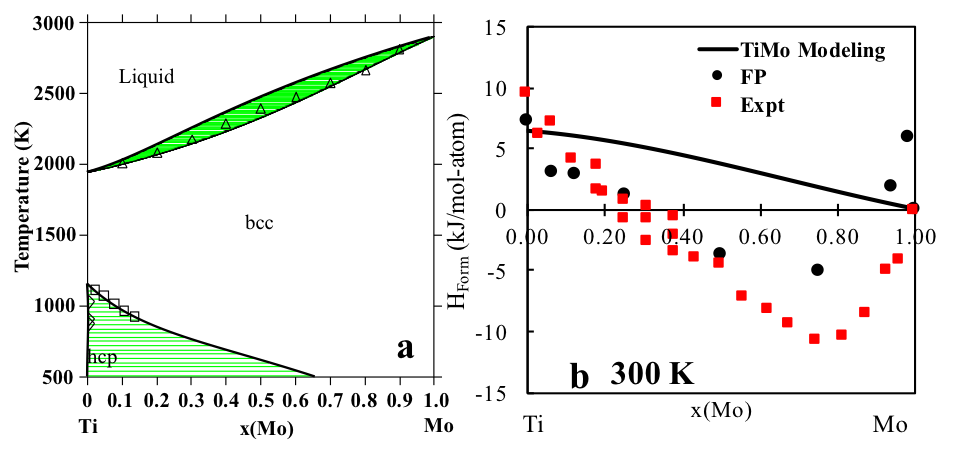
\includegraphics[width=\textwidth]{Chapter-3/Figures/TiMo.png}
	\caption{Figure a on the left plots the previously modeled thermodynamic description of the Ti-Mo system versus available experimental data to ensure accuracy \cite{Ansara1998,Murray1981}. Figure b on the right plots the enthalpy of formation of the bcc phase predicted by the previous thermodynamic modeling (solid line) at 300 K versus the present first-principles calculations (circles) at 0 K.}
	\label{Ch3-figure:TiMo}
\end{figure}
%%%

\newpage
%%%
\begin{figure}[H]
	\centering
	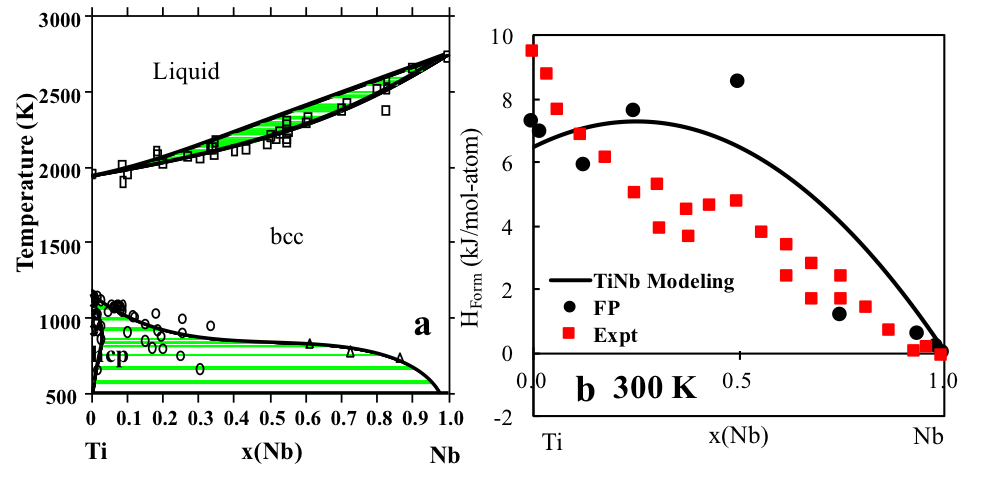
\includegraphics[width=\textwidth]{Chapter-3/Figures/TiNb.png}
	\caption{Figure a on the left plots the previously modeled thermodynamic description of the Ti-Nb system versus available experimental data to ensure accuracy \cite{Zhang2001,Kumar1994}. Figure b on the right plots the enthalpy of formation of the bcc phase predicted by the previous thermodynamic modeling (solid line) at 300 K versus the present first-principles calculations (circles) at 0 K.}
	\label{Ch3-figure:TiNb}
\end{figure}
%%%

\newpage
%%%
\begin{figure}[H]
	\centering
	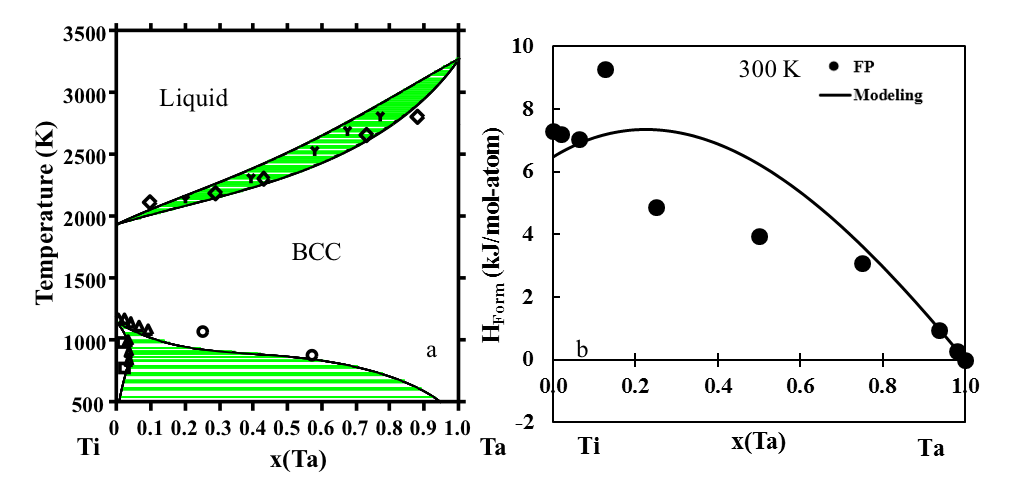
\includegraphics[width=\textwidth]{Chapter-3/Figures/TiTa.png}
	\caption{Figure a on the left plots the previously modeled thermodynamic description of the Ti-Ta system versus available experimental data to ensure accuracy \cite{Ansara1998,Murray1987}. Figure b on the right plots the enthalpy of formation of the bcc phase predicted by the previous thermodynamic modeling (solid line) at 300 K versus the present first-principles calculations (circles) at 0 K.}
	\label{Ch3-figure:TiTa}
\end{figure}
%%%

\newpage
%%%
\begin{figure}[H]
	\centering
	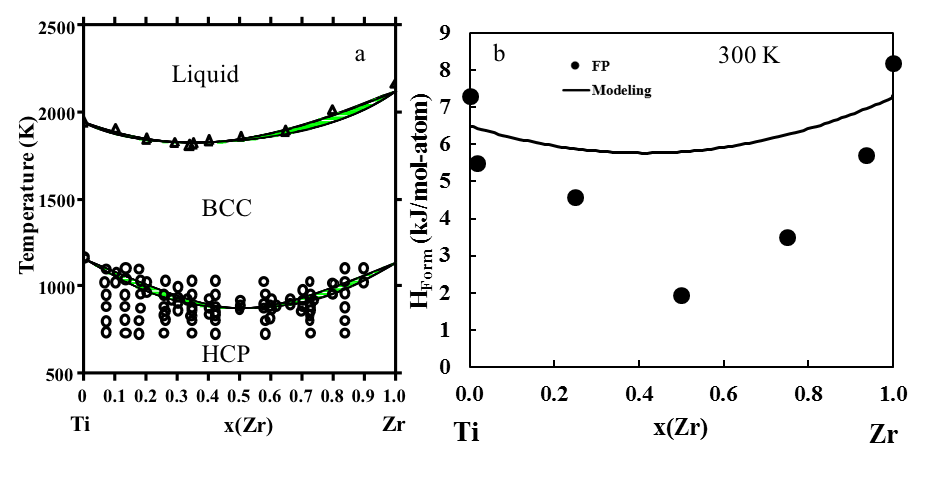
\includegraphics[width=\textwidth]{Chapter-3/Figures/TiZr.png}
	\caption{Figure a on the left plots the previously modeled thermodynamic description of the Ti-Zr system versus available experimental data to ensure accuracy \cite{Kumar1994a}. Figure b on the right plots the enthalpy of formation of the bcc phase predicted by the previous thermodynamic modeling (solid line) at 300 K versus the present first-principles calculations (circles) at 0 K.
	}
	\label{Ch3-figure:TiZr}
\end{figure}
%%%

\newpage
%%%
\begin{figure}[H]
	\centering
	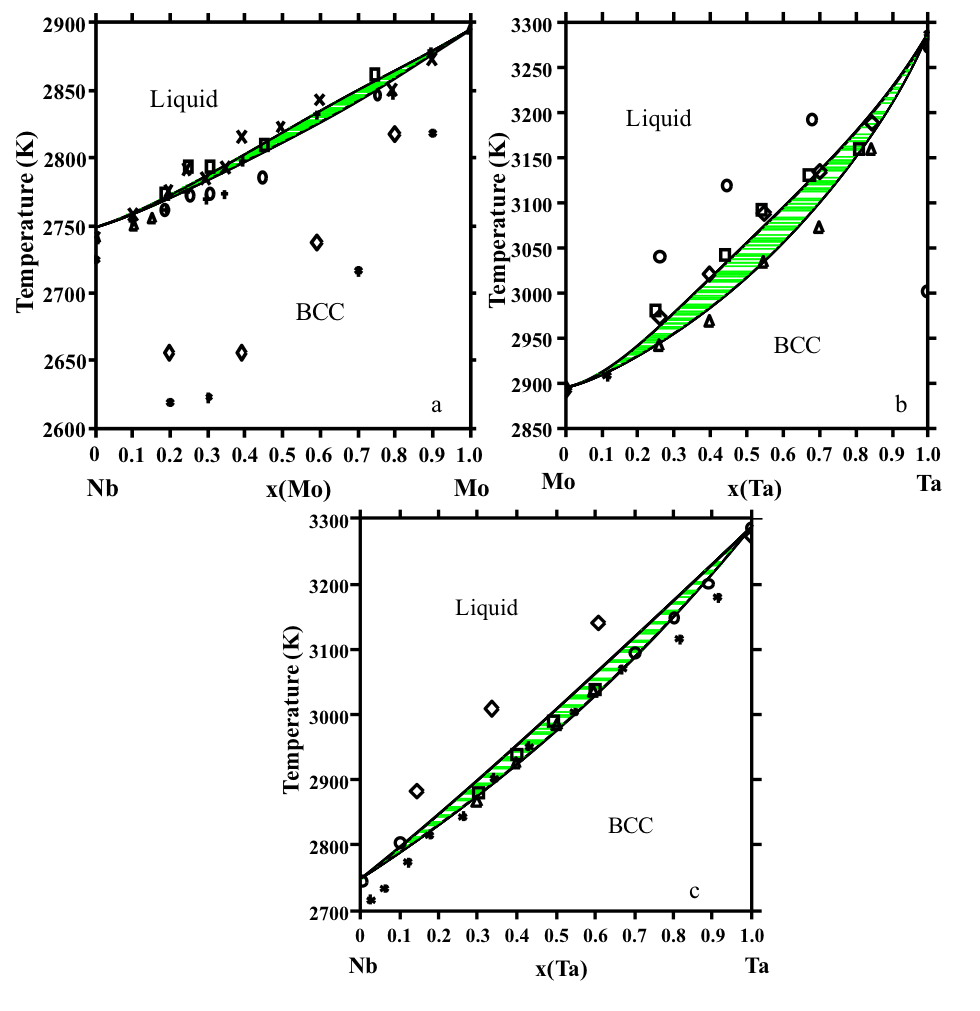
\includegraphics[width=\textwidth]{Chapter-3/Figures/binary1.png}
	\caption{The previously modeled thermodynamic descriptions of the Mo-Nb (a) \cite{Xiong2004}, Mo-Ta (b) \cite{Xiong2004} and Nb-Ta (c) \cite{Xiong2004} binary systems are evaluated by comparing with available phase boundary experimental data.}
	\label{Ch3-figure:binary1}
\end{figure}
%%%

\newpage
%%%
\begin{figure}[H]
	\centering
	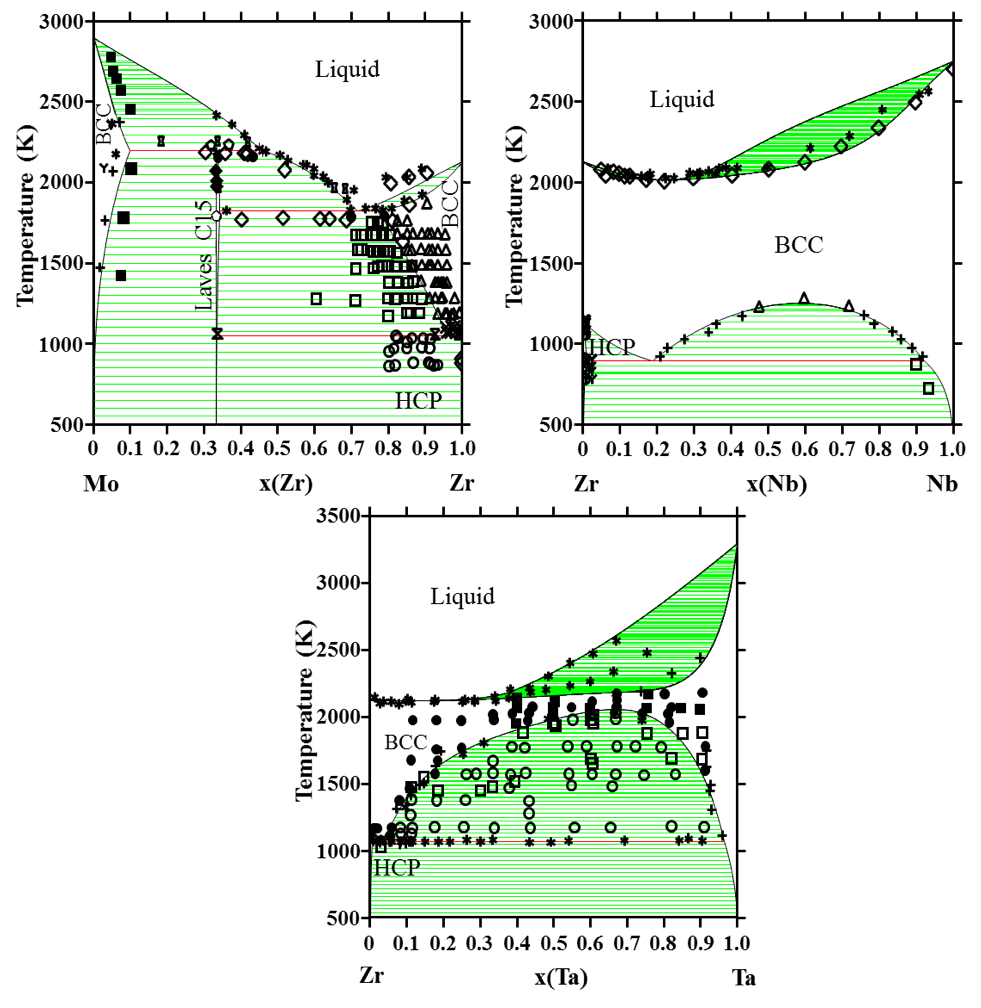
\includegraphics[width=\textwidth]{Chapter-3/Figures/binary2.png}
	\caption{The previously modeled thermodynamic descriptions of the Mo-Zr \cite{Perez2003}, Nb-Zr \cite{Guillermet1991,Abriata1982} and Ta-Zr \cite{Guillermet1995} binary systems are evaluated for accuracy by comparing the available experimental phase boundary data.}
	\label{Ch3-figure:binary2}
\end{figure}
%%%

\newpage
%%%
\begin{figure}[H]
	\centering
	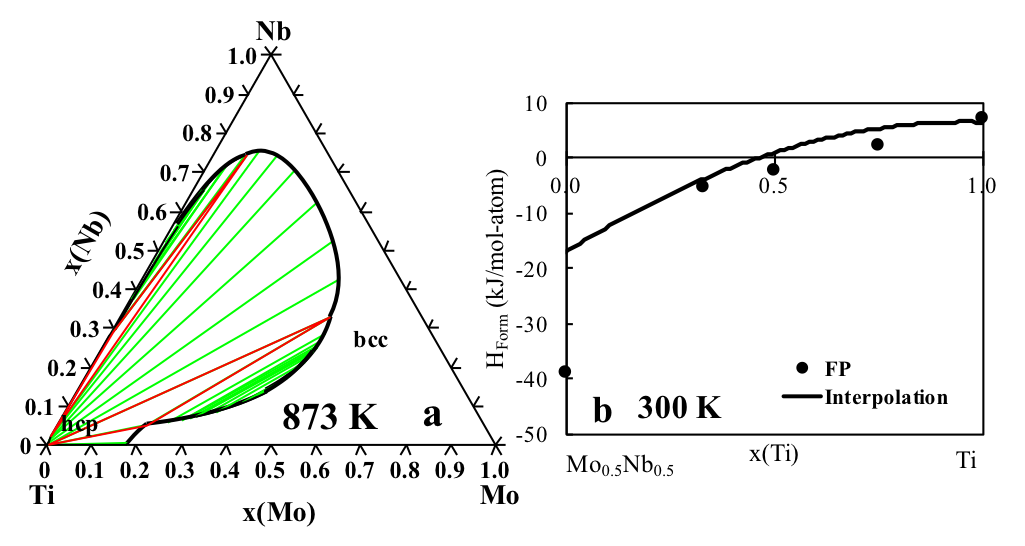
\includegraphics[width=\textwidth]{Chapter-3/Figures/TiMoNb.png}
	\caption{Figure a) on the left is a binary interpolation of the isothermal section of Ti-Mo-Nb plotted at 873 K. Figure b) plots the present calculations (circles) and binary interpolation (solid black line) of the enthalpy of formation of the bcc phase.}
	\label{Ch3-figure:TiMoNb}
\end{figure}
%%%

\newpage
%%%
\begin{figure}[H]
	\centering
	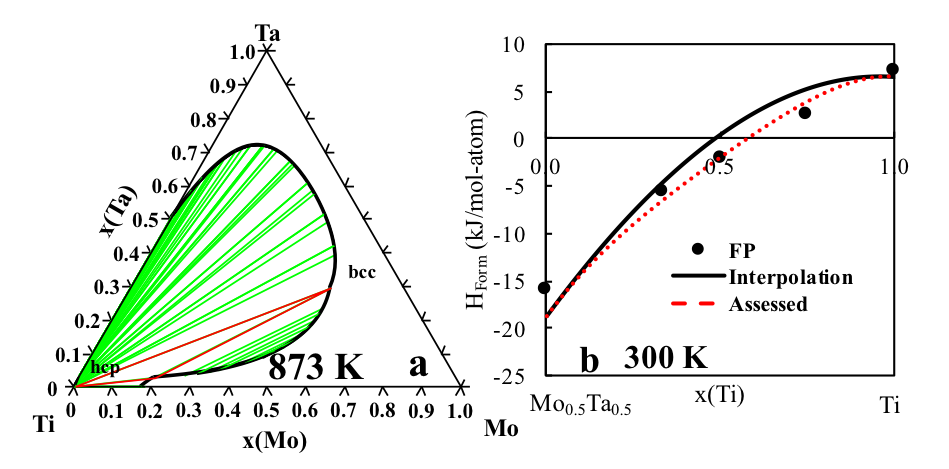
\includegraphics[width=\textwidth]{Chapter-3/Figures/TiMoTa1.png}
	\caption{Figure a) on the left is a binary interpolation of the isothermal section of Ti-Mo-Ta plotted at 873 K. Figure b) plots the present calculations (circles), binary interpolation (solid black line) and ternary assessed (red dotted line) enthalpy of formation of the bcc phase.}
	\label{Ch3-figure:TiMoTa1}
\end{figure}
%%%

\newpage
%%%
\begin{figure}[H]
	\centering
	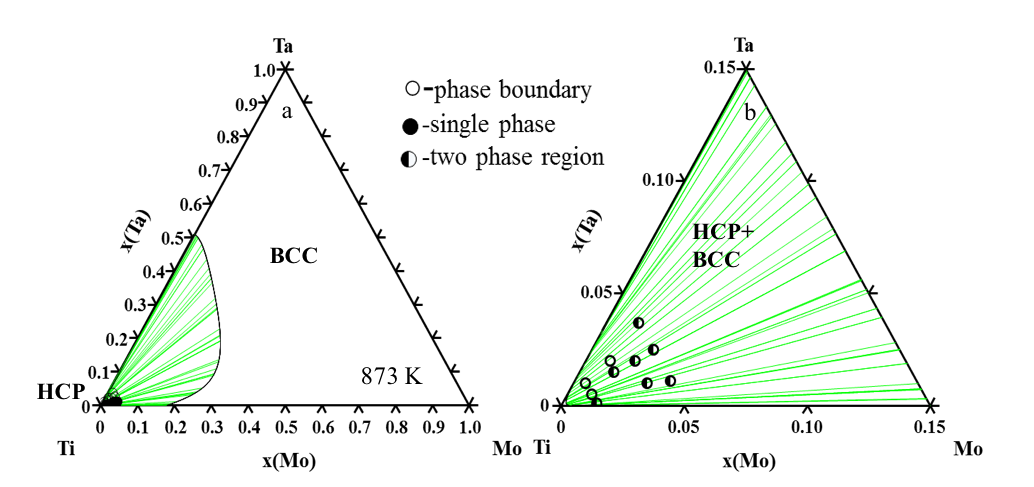
\includegraphics[width=\textwidth]{Chapter-3/Figures/TiMoTa2.png}
	\caption{Figure a) on the left is the isothermal plot of Ti-Mo-Ta at 873 K after evaluation of the ternary interaction parameters. Figure b) on the right is zoomed in to show the comparison with the experimental data \cite{Nikitin1971}.}
	\label{Ch3-figure:TiMoTa2}
\end{figure}
%%%

\newpage
%%%
\begin{figure}[H]
	\centering
	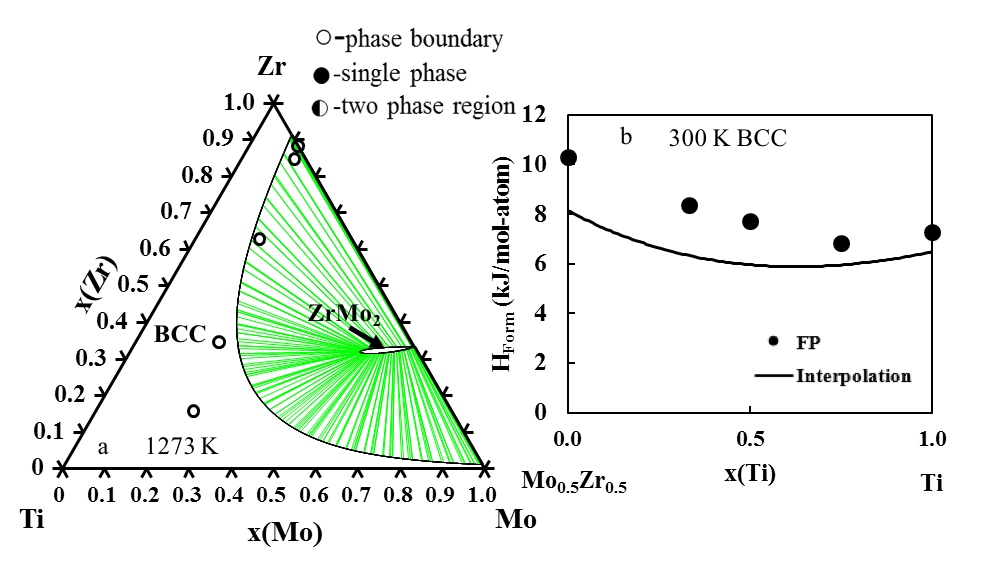
\includegraphics[width=\textwidth]{Chapter-3/Figures/TiMoZr.png}
	\caption{Figure a) on the left is a binary interpolation of the isothermal section of Ti-Mo-Zr plotted at 1273 K with experimental phase data obtained at the same temperature \cite{Kar2008,Prokoshkin1967}. Figure b) plots the present calculations (circles) and binary interpolation (solid black line) of the enthalpy of formation of the bcc phase.}
	\label{Ch3-figure:TiMoZr}
\end{figure}
%%%

\newpage
%%%
\begin{figure}[H]
	\centering
	\includegraphics[width=\textwidth]{Chapter-3/Figures/TiNbTa1.png}
	\caption{Figure a) on the top left is a binary interpolation of the isothermal section of Ti-Nb-Ta plotted at 673 K. Figure b) is a binary interpolation of the isothermal section of Ti-Nb-Ta at 823 K. Both binary interpolations are compared with experimental phase boundary data \cite{Na2001}. Figure c) plots the present calculations (circles), binary interpolation (solid black line) and ternary assessed (red dotted line) enthalpy of formation of the bcc phase.}
	\label{Ch3-figure:TiNbTa1}
\end{figure}
%%%

\newpage
%%%
\begin{figure}[H]
	\centering
	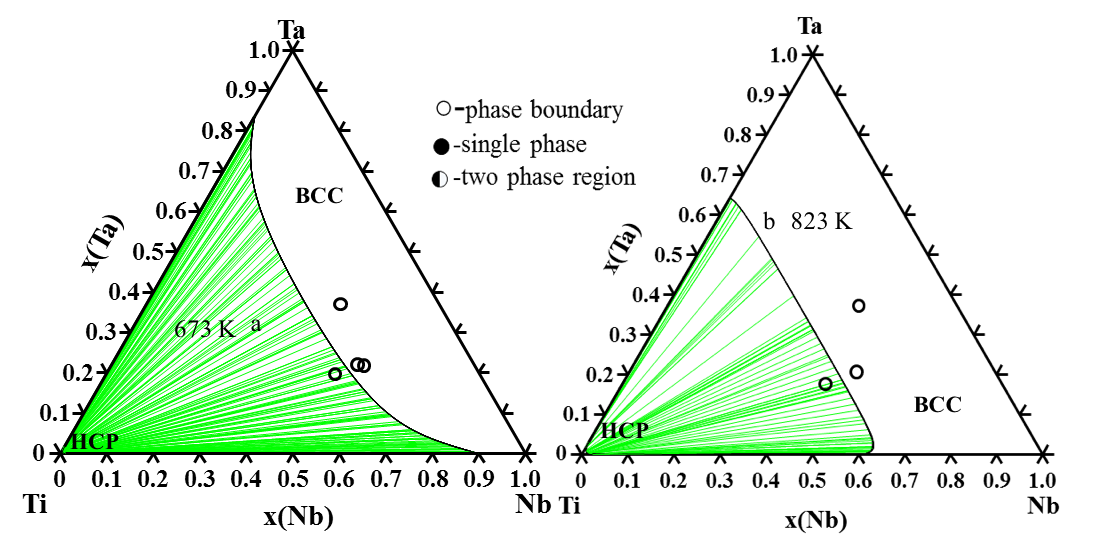
\includegraphics[width=\textwidth]{Chapter-3/Figures/TiNbTa2.png}
	\caption{Figure a) on the left is the isothermal plot of Ti-Nb-Ta at 673 K after evaluation of the ternary interaction parameters. Figure b) is the evaluated isothermal plot of Ti-Nb-Ta at 823 K. Both plots have experimental phase boundary data \cite{Na2001}.}
	\label{Ch3-figure:TiNbTa2}
\end{figure}
%%%

\newpage
%%%
\begin{figure}[H]
	\centering
	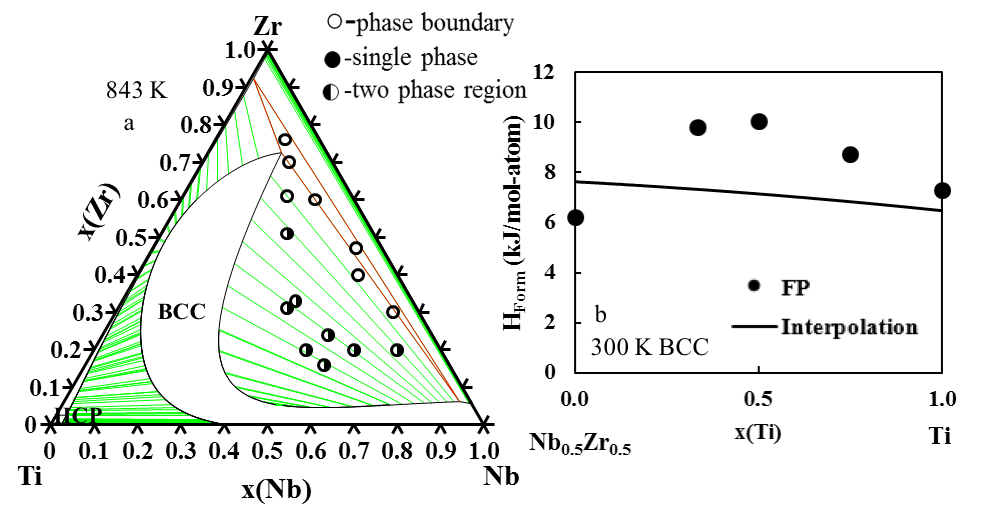
\includegraphics[width=\textwidth]{Chapter-3/Figures/TiNbZr.png}
	\caption{Figure a) on the left is a binary interpolation of the isothermal section of Ti-Nb-Zr plotted at 843 K with experimental phase data \cite{Tokunaga2007}. Figure b) plots the present calculations (circles) and binary interpolation (solid black line) of the enthalpy of formation of the bcc phase.}
	\label{Ch3-figure:TiNbZr}
\end{figure}
%%%

\newpage
%%%
\begin{figure}[H]
	\centering
	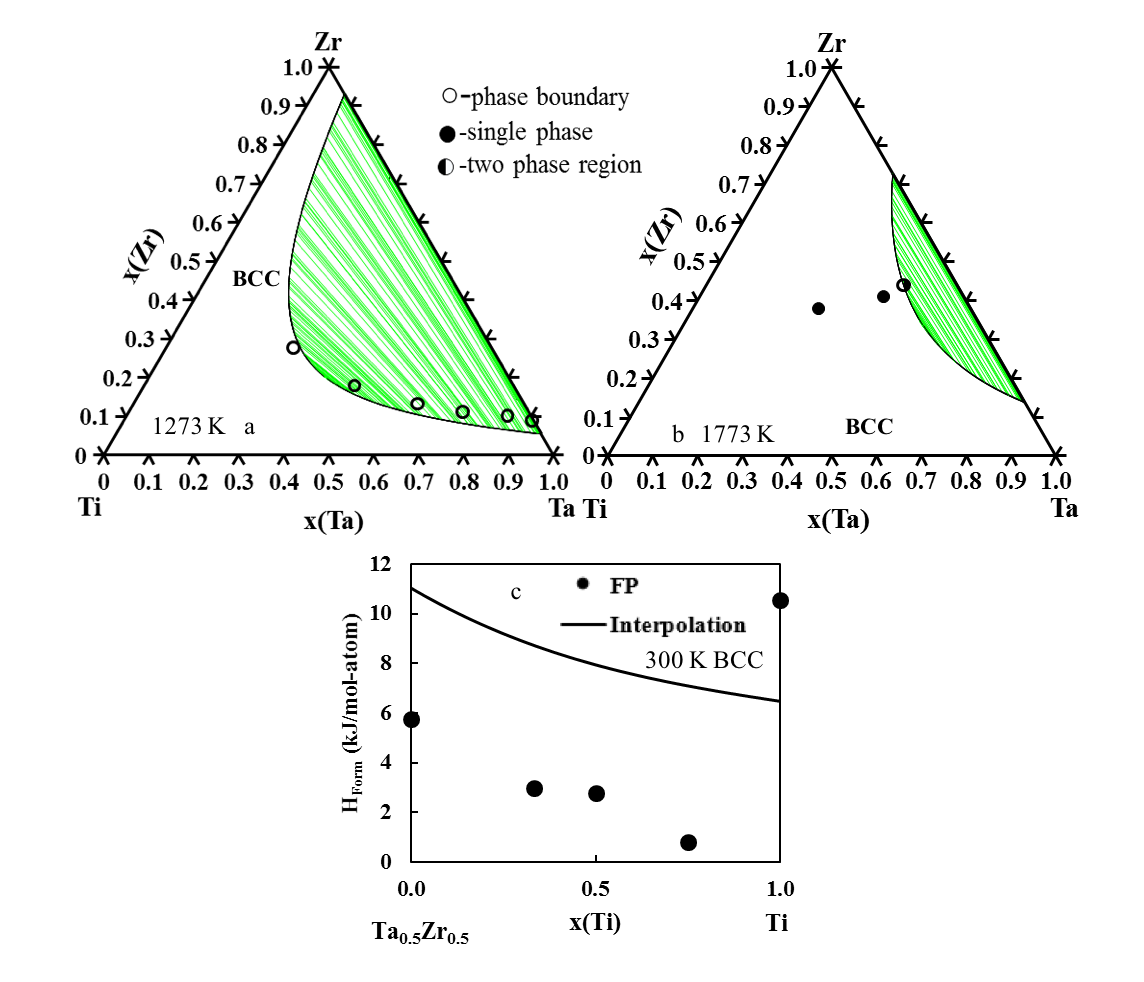
\includegraphics[width=\textwidth]{Chapter-3/Figures/TiTaZr1.png}
	\caption{Figure a) on the top left is a binary interpolation of the isothermal section of Ti-Ta-Zr plotted at 1273 K. Figure b) is a binary interpolation of the isothermal section of Ti-Ta-Zr at 1773 K. Both binary interpolations are compared with experimental data \cite{Lin1996,Hoch1964}. Figure c) plots the present calculations (circles) and binary interpolation (solid black line) for the enthalpy of formation of the bcc phase.}
	\label{Ch3-figure:TiTaZr}
\end{figure}
%%%